\documentclass[11pt]{article}

\usepackage{common}
\usepackage{booktabs}
\title{Practical 2: Malware Classification}
\author{70939479 \\ Jazz  \\ Zhang, Xihan(91297655) \\Team JXJ: Jmencab, Xihan, JazzName}
\begin{document}


\maketitle{}



\section{Technical Approach}

The main issue in this classification practical was extracting features. It seemed to us that the randomized feature extraction made little sense in terms of being able to compare the effectiveness of different models on a given data set as it would not be a consistent comparison. The first set of features we extracted was simply the number of system calls made per file. This we then converted to binary and did a classification on the resultant bit vector. This provided results beating the $50\%$ baseline when used with Bernoulli Naive Bayes, Logistic Regression, Extra Tree, Knn, SVM and neural net (multi-layer perceptron). In order to improve upon this, however, we knew that we would need to get more expressive features. 

The next feature that we tried was a per-file, per-system-call count data set. This proved to be much better with all the previously mentioned models that we tried on the simpler data set. We also tried XGBoost on this data set. Our results here were in some cases not as good as with the ostensibly less expressive previous data set. As such, we decided that hyper-parameter tuning was in order.

For each model, $20\%$ data were randomly split as test set to report accuracy and 7-fold cross-validation were performed to tune hyper-parameter on the remaining $80\%$ data. From the raw models(Table 2), we chose ones with better accuracy to tune: (1) Logistic Regression(tuned accuracy:$70\%$): Given the unbalanced class in data, we compared weighted(adjusted by class frequency) vs unweighted ones, and over-all classification accuracy in unweighted($68\%$) ones are surprisingly better weighted ones($39\%$). (2) Extra Tree(tuned accuracy:$89\%$): Performs slightly better than Random Forest($73\%$), thus we tuned ExtraTree($75\%$). With 107 features, we found number of estimators(which control the variance)=60 and the max depth(which control bias of single tree)=50 the best. (3) Neural Network(tuned accuracy:$86\%$): We found 'logistic' activation yield better performance than other 3('identity', 'tanh', 'relu'), best learning rate=0.01, hidden layer size=400 and penalty alpha=0.00001. (4) XGBoost(tuned accuracy:$90\%$): We found 'gbtree' is better than other booster('gblinear', 'dart'), and best max depth=4, n estimators=200, learning rate=0.1. 

This tuning ultimately put us over the edge in terms of beating the $79\%$ baseline set by the bigram data($81\%$). Taking inspiration fr0m a Microsoft Kaggle competition on malware detection, we decided to extend our features to 1,2,3,4-grams and tried combining the resulting csv's containing those n-grams to the per-file, per-system call counts file and running predictions based off that. The new features fitted on XGBoost did give us best score of $83\%$, but combining them with all previous features decreases the score to $82\%$, which motivated us to dive deeper into feature selection and meta-classifier.

Based on the final accuracy after tuning, we choosed XGBoost and ExtraTree as final models to perform feature selection. The first step is to delete junk features with no variance among all class. Then we use feature importance=0 as selection criteria: from the 1068 features(all features we have), Extra Tree filtered out 228 and XGBoost filtered out 568. We found the 568 features selected by XGBoost is less noisy(test and train accuracy more close to each other), so that we go with this 568 features. Since features from1,2,3,4-grams may theoretically have strong collinearity, we drew a heat-map of Pearson coefficients of every pair of features, it surprisingly turns out little collinearity problems(Figure1), we then used p-value $>0.98$ to filtered out 150 features. The model performance on test set was improved from $88\%$(1068 features) to $91\%$(331 features), the accuracy on Camelot, however, rapidly decreased from $82\%$ to $27\%$. Then we built meta-classifier combining prediction from 20 ExtraTrees and 30 XGBoost models to take the final vote, but it still doesn't help improve the score. This result making us believe the class weight in Camelot is different from ours, selecting features based on Training set may lead to strong overfitting.  Thus we also tried over-sample the class with little proportion in the whole data, but that was finished after Camelot freeze, so we didn't have chance to test the performance.


\begin{figure}
\centering
\includegraphics[width=0.5\textwidth]{heatmap_pearson.pdf}
\caption{Heat-map for Pearson correlation coefficients of features}
\label{fig:heatmap_pearson}
\end{figure}

Below are lists showing the models used and the sets of features generated:

  \begin{table}
    \centering
    \begin{tabular}{@{}lll@{}}
     \toprule
      &\multicolumn{1}{c}{Features Generated} \\
      \midrule
      & Total System Calls\\
      & Per-system-call Counts \\
      & Byte Size \\
      & Bigram \\
      & 3-gram  \\
      & 4-gram \\
      \bottomrule
    \end{tabular}
    \caption{Feature sets generated from input data.}
  \end{table}
  
    \begin{table}
    \centering
    \begin{tabular}{@{}lll@{}}
     \toprule
      &\multicolumn{1}{c}{Models Used} \\
      \midrule
      & \\
      & Weighted Logistic Regression (sklearn.linear model)\\
      & Unweighted Logistic Regression (sklearn.linear model) \\
      & SVM (sklearn) \\
      & Extra Tree (sklearn.ensemble)\\
      & Random Forest (sklearn.ensemble)\\
      & Bernoulli Naive Bayes (sklearn.naive bayes)\\
      & Knn (sklearn.neighbors)\\
      & Neural Network (sklearn.neural network)\\
      & XGBoost (xgboost.sklearn)\\
      \bottomrule
    \end{tabular}
    \caption{Models used}
  \end{table}
 
\section{Results}
\begin{figure}
\centering
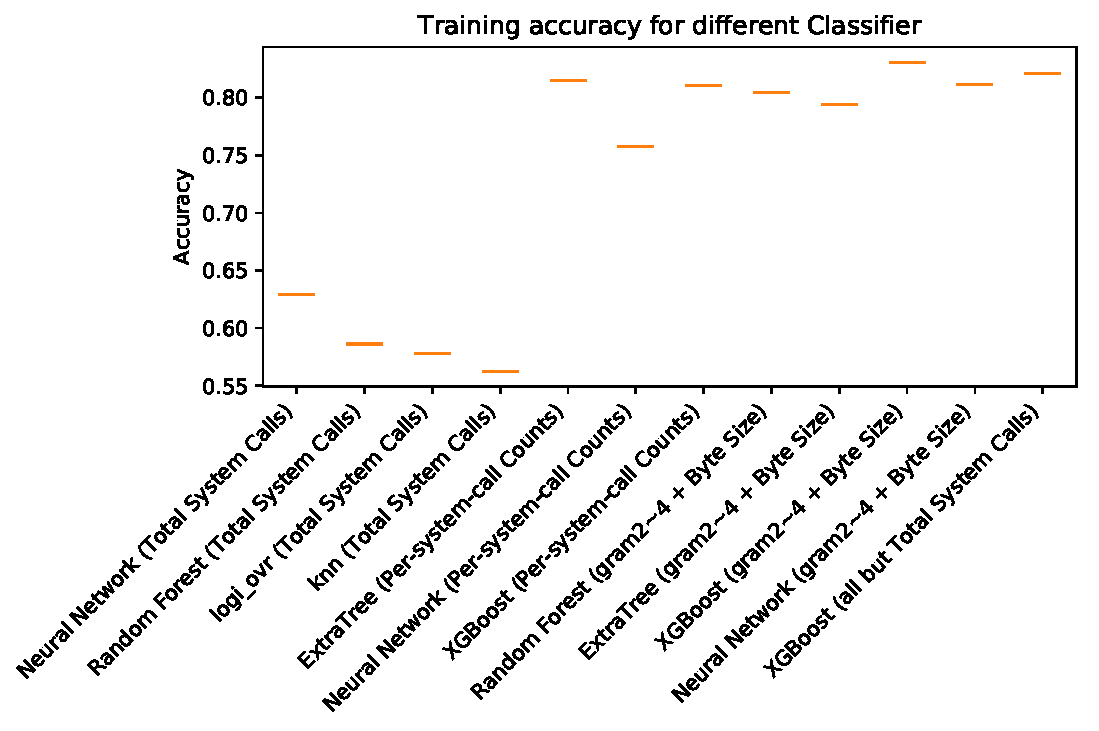
\includegraphics[width=\textwidth]{Results.pdf}
\caption{Camelot Score for different models and features}
\label{fig:Results}
\end{figure}
This section should report on the following questions: 

\begin{itemize}
\item Did you create and submit a set of
  predictions? 
  

\item  Did your methods give reasonable performance?  
\end{itemize}

\noindent You must have \textit{at least one plot or table}
that details the performances of different methods tried. 
Credit will be given for quantitatively reporting (with clearly
labeled and captioned figures and/or tables) on the performance of the
methods you tried compared to your baselines.

% Julio, this plot maybe more efficient than table, but the submission results are not all we have, if you have new idea on how to cluster them, I can help plot this figure after 18:00 today, I can also go to Currier House if necessary 





\section{Discussion} 


End your report by discussing the thought process behind your
analysis. This section does not need to be as technical as the others 
but should summarize why you took the approach that your did. Credit will be given for:

  \begin{itemize}
  \item Explaining the your reasoning for why you seqentially chose to
    try the approaches you did (i.e. what was it about your initial
    approach that made you try the next change?).  
  \item Explaining the results.  Did the adaptations you tried improve
    the results?  Why or why not?  Did you do additional tests to
    determine if your reasoning was correct?  
  \end{itemize}
 

\end{document}


